\subsection{Simulated event samples}

To perform a precise measurement of the angular distributions and asymmetries described in Section~\ref{sec:ch02} with the purpose of explore the possible presence of anomalous couplings in the $Wtb$ vertex, accurate MC models predicting the characteristics of the expected data are needed for both the signal and SM background precesses. All simulation samples are passed through the MC simulation of ATLAS detector~\cite{Aad:2010ah} based on \textsc{Geant4}~\cite{Agostinelli:2002hh}. Since the final observable is an angular distribution, which is highly sensitive to kinematic mismodelling, special care must be taken in this analysis~\cite{MorenoLlacer:2014tca}.


The single-top-quark production in the $t$-channel sample is produced combining the NLO MC generator \textsc{Powheg}~\cite{Alioli2010} and the general purpose MC generator \textsc{Pythia8}~\cite{Sjostrand:2006za} for the parton shower, fragmentation and the underlying event. The simulation includes both the $q+b \rightarrow q'+t$ and $q+g \rightarrow q' +t +\bar{b}$ diagrams (Figure \ref{Fig:FeynmanSingTopProd}-b).



The background processes are those which mimic the experimental signature of $t$-channel single-top-quark events. These can be classified in four main groups:
\begin{itemize}
\item Top quark pair ($t\bar{t}$), $s$-channel and $Wt$-channel: production of top quarks via strong interactions and other channels of electroweak production.
\item $W$+jets: production of a real $W$ boson in association with heavy- or light-flavour jets.
\item $Z$+jets: electroweak production of single $Z$ boson and diboson.
\item Multijet: events from QCD multijet production where one jet is identified as a lepton and a mismeasurement creates large $E_T^{miss}$. %"fake lepeton"
\end{itemize}
%include the production of $W$ and $Z$ bosons ($W$+jets and $Z$+jets), top quark production (both $t\bar{t}$ and single top in the $s$-channel) and diboson production. 

The $W$ and $Z$ bosons are simulated with \textsc{Sherpa}2.1.1 generator~\cite{5-ref24}, in which matrix elements up to two partons are calculated at NLO while LO calculations are used for 3 and 4 partons. The CT10 parton distribution function (PDF) set is used. The $W$+jets and $Z$+jets processes are normalised to their NNLO prediction. The backgrounds $t\bar{t}$, single-top $s$-channel and $Wt$ processes, are simulated using \textsc{Powheg} generator with \textsc{Pythia8} for the parton shower, fragmentation and the underlying event as it has been done for the signal $t$-channel events. Diboson production, including $WW$ , $WZ$ and $ZZ$ is simulated with Sherpa2.1.1 with the CT10 PDF set. In Table~\ref{Table:Generator} is shown how these processes are generated.

\begin{table} [htb]
\begin{center}
\renewcommand{\arraystretch}{1.2}
\begin{tabular}{|l l l|}
\hline
Process & Generator & PDFs \\
\hline
\textbf{Single top} & & \\
$t$-channel & \textsc{Powheg}+\textsc{Pythia} & CT10 \\
$s$-channel & \textsc{Powheg}+\textsc{Pythia} & CT10 \\
$Wt$ & \textsc{Powheg}+\textsc{Pythia} & CT10 \\
\hline
\textbf{$t\bar{t}$} & \textsc{Powheg}+\textsc{Pythia} & CT10 \\
\textbf{$W\rightarrow l \nu +jets$} & \textsc{Powheg}+\textsc{Pythia} & CT10 \\
\textbf{$Z \rightarrow \nu \nu, ll +jets$} & \textsc{Powheg}+\textsc{Pythia} & CT10 \\
\hline
\textbf{Diboson} & & \\
$WW$ & \textsc{Sherpa} & CT10 \\
$WZ$ & \textsc{Sherpa} & CT10 \\
$ZZ$ & \textsc{Sherpa} & CT10 \\
\hline
%\textbf{QCD Multijet} & & \\
%jj & \textsc{Pythia} & NNPDF23\_lo \\
%\hline
\end{tabular}
\caption{List of MC generators and PDFs used for the different signal and background processes that have been simulated.}
\label{Table:Generator}
\end{center}
\end{table}

The multijet background is the only process that is not determined though a MC simulation, for this events the data-driven matrix method has been used~\cite{Aaboud:2016ymp}. This method~\cite{ATLAS-CONF-2014-058} allows to estimate the number of multijet background events in the signal region by deriving the true composition of the data sample in terms of prompt (real) and fake leptons from its observed composition in terms of tight (signal selection) and loose leptons. The loose lepton selection consist of identical requirements as for those applied to the tight signal sample but relaxing the identification criteria on the leptons, electrons or muons, mainly relaxing the lepton isolation requirements. The stringent tight selection is a subset of the lax loose selection. The number of multijet events $N_{fake}^{tight}$ passing the signal requirements can be expressed as:
\begin{equation*}
N_{fake}^{tight} = \frac{\epsilon_{fake}}{\epsilon_{real}}(N^{loose}_{data} \cdot \epsilon_{real} - N^{tight}_{data})
\end{equation*}
where $\epsilon_{real}$ real and $\epsilon_{fake}$ are the efficiencies for real and fake loose leptons being selected as tight leptons, $N^{loose}_{data}=N^{loose}_{real}+N^{loose}_{fake}$ is the number of selected events in the loose sample, and $N^{tight}_{data}=N_{real}^{tight}+N_{fake}^{tight}$ is the number of selected events in the signal sample. 
The fake-lepton efficiencies are determined from a data sample dominated by non-prompt and fake-lepton background events. The real-lepton efficiencies are also estimated from collision data using a ``tag-and-probe” method in $Z \rightarrow ee$ events.








\subsection{Object reconstruction}\label{subseb:Reco}
The objects to be reconstructed in this analysis are the electrons, jets and $E_T^{miss}$. The electron and the neutrino ($E_T^{miss}$) come from the decay of the $W$ boson and the jets arise from the quarks, these are the elements present at the final state in the top quark production and decay in the $t$-channel, as can be seen in Figure~\ref{Fig:FeynmTotal}.
\begin{figure}[htb]
\centering
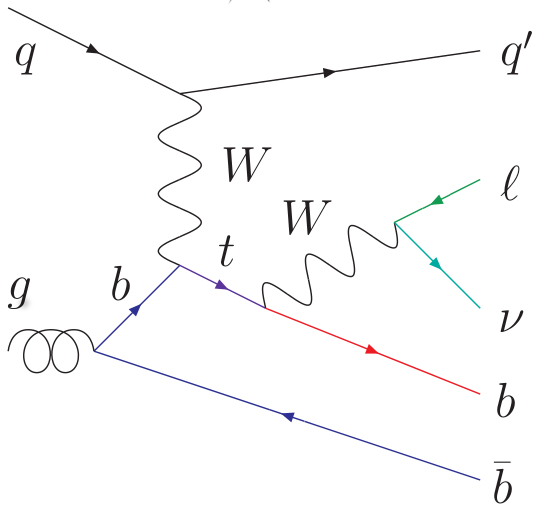
\includegraphics[width=0.35\textwidth]{/afs/ific.uv.es/user/p/pamarag/public/RedaccionTFM/Figuras/tChannelFeynmanTOTAL.jpg}
\caption{Representative Feynman diagram for $t$-channel single-top-quark production and decay.}
\label{Fig:FeynmTotal}
\end{figure}

% ELECTRONS
Electron candidates are identified as clusters of energy deposited in the electromagnetic calormeter with a well measured track~\cite{Aad:2014fxa}~\cite{ATLAS:2014wga}. They are required to have a $p_T > 30$~GeV and the cluster must yield in the region defined by the pseudorapidity range of $|\eta_{clus}|<2.47$, excluding the region $1.37<|\eta_{clus}|<1.52$. In order to reduce background events in which a hadronic jet is misidentified as a prompt electron or electrons from the decay of heavy quarks, isolation criteria are applied. These criteria are optimised such that, by adjusting the isolation threshold, the selection efficiency of the isolation criteria is uniform across the $\eta$ of the electron. This efficency increases from 90\% for $p_T = 25$~GeV to 99\% for $p_T = 60$~GeV~\cite{Aaboud:2016ymp}. In addition, all tracks (excluding the track belonging to the electron) in a cone of size $\Delta R = \sqrt{(\Delta \eta)^2+(\Delta \phi)^2} = 0.3$ around the electron direction have a restriction of $p_T$ below a threshold dependig on the electron tranverse momentum. Finally, a calorimeter isolation in a cone of size 0.2 around the electron is required~\cite{Aaboud:2016pbd}.

% JETS
Jets are reconstructed with the so called anti-$k_t$ algorithm~\cite{Cacciari:2008gp} with a radius parameter\footnote{The $R$ in distance parameter $d_{ij} = min(k_{T,i}^{2P},k_{T,j}^{2P})\frac{R^2_{ij}}{R^2}$, being $R_{ij}$ the distance between to objects in the $\eta$ -- $\phi$.} of 0.4. This method is a successive recombination algorithm that inverts the parton shower be combining the constituents of the jet according to distance criteria weighted by relative transverse momentum. The calibration is done using a combination of data and a simulation depending in the energy and the $|\eta|$~\cite{TheATLAScollaboration:2015soq}. Only jets with $p_T > 30$~GeV and $|\eta|<3.5$ are accepted. The rapidity range is determined using a region dominated by $W$+jets and by requiring a good agreement between simulated a measured data.

When there are jets close to an electron in the $\Delta R < 0.2$ range, the closest jet is removed because both, the electron and jet, are likely to correspond to the same physical object. The remaining electron candidates overlapping with jets within $\Delta R < 0.4$ are subsequently rejected. 

To discriminate between jets from hard-scatter processes and those from pile-up, the jet vertex tagger (JVT) is used as a discriminant~\cite{Aad:2015ina}. It is constructed from tracking and vertex information using a two-dimensional likelihood method. The JVT variable is required to be more than 0.64 for jets with $p_T > 50$~GeV and $|\eta|<2.4$, corresponding to an efficiency of 92\% and a misidentification rate of 2\%.

% b-TAGGING
In this analysis it is important to identify the $b$-jets\footnote{Jets corresponding to the hadronization of a $b$-quark.}. With that purpose we use a $b$-tagging algorithm, based on boosted decisions trees which is optimised to reject $c$-jets as well as light quark jets. This algorithm can only be applied to jets with the coverage of the ID. The $b$-tagging efficiency is extracted from $t\bar{t}$ simulated events and it is 60\%. 0.06 \% of light-quark jets and 4.7 \% of $c$-quark jets are mistagged as $b$-quark jets~\cite{Aaboud:2016ymp}.
%Inner Detector = $|\eta|<2.5$.

% E_T^{MISS}
The magnitude of the missing transverse momentum is a measure of the momentum imbalance in the plane transverse to the beam axis due to the escaping neutrinos. It is defined as $E_T^{miss}= |\overrightarrow{E_T}^{miss}|$, where the vector $\overrightarrow{E_T}^{miss}$ is obtained using the reconstructed three-dimensional calorimeter energy clusters associated with the selected jets together with either the calibrated calorimeter energy cluster associated with an electron or the $p_T$ of a muon track. Contributions from soft particles not associated with the identified ones, are accounted for using tracks associated to vertex but not associated with a jet or electron~\cite{Aaboud:2016ymp}.


\subsection{Trigger requirements and event preselection}

The experimental signature of $t$-channel single top-quark events in the single lepton channel consists of one isolated charged lepton from the $W$-boson decay, large $E_T^{miss}$ due to the neutrino coming from the leptonically decaying $W$ boson, exactly two jets and one of them identified as likely to be originated from the fragmentation
of the $b$-quark coming from the top-quark decay. Then, the remaining jet would be the forward jet originated by the fragmentation of the spectator quark.

In this master thesis we have analysed only the electron channel due to technical reasons of availability of the analysis samples at the time of the research work was developed. Along with the trigger requirements, the preselection requirements summarised in Table~\ref{Table:PreselectionCuts} are applied. This set of cuts is implicitly applied in all the further set of cuts used in this work.

Only events passing the single-electron trigger are considered~\cite{Aad:2014sca}~\cite{Aaboud:2016ymp}. The L1 (subsection~\ref{subsec:trigg}) requirement demands a $E_T$ deposit above 20 GeV with a reduced calorimetric granularity being considered at this stage. Events in the electron channel are triggered by a calorimeter cluster matched to a track, and the trigger electron object is required to have either $E_T >60$~GeV or $E_T >24$~GeV and satisfy some isolation criteria. Only events containing exactly one isolated charged lepton with $p_T > 30$~GeV and $|\eta|<2.5$ are accepted. Candidate events must have exactly two jets satisfying the criteria described in Section~\ref{subseb:Reco}. Jets reconstructed in the range $2.75<|\eta|<3.5$, covering the endcap-forward calorimeter transition region, must have $p_T > 35$~GeV. One of the selected jets is required to be identified ($b$-tagged) as a $b$-jet.



In order to reject a part of the multijet background events, which are characterised by low $E_T^{miss}$ and the transverse mass of the $W$-boson $m_{T}(W)$\footnote{Defined as $m_{T}(W)=\sqrt{2p_T^l E_T^{miss} [1-\cos(\phi^l - \phi^{E_T^{miss}})]}$, being $p_T^l$ the transverse momentum of the lepton, $\phi^l$ its azimuthal angle and $\phi^{E^{miss}_T}$ the azimuthal angle of the $E_T^{miss}$.}, the event selection requires $E_T^{miss}<30$~GeV and $m_{T}(W) > 50$~GeV. To further suppress the multijet background a requirement on the $p_T$ of the charged lepton and the azimuthal angle between the charged lepton and jet is applied~\cite{Aaboud:2016ymp}~\cite{Aad:2014fwa}:
%\begin{equation*}
%p_T(l) > \text{max} \left(30\text{ GeV, 40 GeV}\cdot \frac{\Delta \phi(j_1, l)}{\pi} \right)
%\end{equation*}
\begin{equation*}
p_T(l) > 40\left(\frac{|\Delta \phi(j_1, l)|-1}{\pi -1} \right) \text{GeV,}
\end{equation*}
where $l$ denotes the charged lepton and $j_1$ the reconstructed jet with the highest $p_T$.


A dilepton veto is applied to reject dileptonic sources of background, mainly $t\bar{t}$ dileptonic events. Therefore, contributions from processes with two isolated leptons in the final state are suppressed by rejecting any event with an additional electron or muon as defined above satisfying $p_T > 10$~GeV. This cuts are summarised in Table~\ref{Table:PreselectionCuts}.





%The L1 (subsection~\ref{subsec:trigg}) requirement demands a transverse energy deposit above 20 GeV with a reduced calorimetric granularity being considered at this stage. %At the HLT, a track is matched to the full granularity of the calorimeter as well as tracking information are available and the reconstructed calorimeter cluster.
%The trigger electron object is then required to be isolated and to have $E_T > 24$~GeV. The electron channel is also triggered on events with an $E_T$-threshold of 60 GeV and 120 GeV at the HLT but without isolation requirement in that case.



%Those events are triggered by a calorimeter cluster matched to a track the trigger electron object is required to have either $E_T > 60$~GeV or $E_T > 24$~GeV and satisfy isolation criteria.

%The experimental signature of the single lepton channel events is one isolated lepton from the W boson decay, large missing transverse momentum, and one jet identified as likely to have originated from a $b$-quark. Therefore, preselected events are required to contain one tight lepton with transverse momentum\footnote{The momentum in the plane perpendicular to the beam axis: $p_T=\sqrt{p_x^2 + p_y^2}$, being $p_x^2$ and $p_y^2$ the momentum in the $X$ and $Y$ axis as defined in section~\ref{subsec:ATLAS}. Momentum conservation in the $XY$-plane requires that the vectorial sum of the transverse momenta of all final-state particles is (approximately) zero as well.} $p_T > 30$~GeV, one jet with $p_T > 30$~GeV and required to be $b$-tagged, $E_T^{miss} > 50$~GeV and, in order to reject background events, both the $E_T^{miss}$ and the transverse mass of the $W$-boson $m_{T}(W)=\sqrt{2p_T^l E_T^{miss} [1-\cos(\phi^l - \phi^{E_T^{miss}})]}$ are required to be larger than 30~GeV. The upper index $l$ refers to the lepton. A di-lepton veto is applied.
%In order to reject background events, both the $E_T^{miss}$ and the transverse mass of the $W$-boson $m_{T}(W)=\sqrt{2p_T^l E_T^{miss} [1-\cos(\phi^l - \phi^{E_T^{miss}})]}$ are required to be larger than 30~GeV. The upper index $l$ refers to the lepton.



\begin{table} [htb]
\begin{center}
%\resizebox{0.95\textwidth}{!}
\caption{Preselection requirements. These cuts are implicitly applied in all further selections.}
\label{Table:PreselectionCuts}
\end{center}
\end{table}


After imposing the preselection cuts of Table~\ref{Table:PreselectionCuts} over the 13~TeV simulated samples for $t$-channel single-top-quark production with the leptonic decay of the top quark to an electron, we get the event yields presented at Table~\ref{Table:PreselectionEventYields}. Given the small fraction of signal events in the dataset at preselection level, further requirements are applied to separate the signal from the background. From now on, the errors on the event yields presented at Tables \ref{Table:PreselectionEventYields}, \ref{Table:8&13}, \ref{Table:mlbevents}, \ref{Table:mtopevents}, \ref{Table:ABCtriang}, \ref{Table:MjtHtMisc} and \ref{Table:FINAL} account only for the statistical precision of the MC.


\begin{table} [htb]
\begin{center}
%\resizebox{0.95\textwidth}{!}{%<---- To fit the table
\begin{tabular}{|c|c|c|c|c|} 
 \hline
 Process & Event yield & Bkg fraction \\ \hline
 $t$-channel & $41154 \pm 127 $ & - \\ 
 $Z$-jet, diboson & $10217 \pm 239 $&  3.0\% \\ 
 $W$+jets & $151047 \pm  1748$ & 44.5\%\\
 $t\bar{t}$& $119770 \pm 230$ & 35.2\%\\
 $Wt$ s-channel & $27580 \pm 123$ & 8.1\% \\
 Multijet&$31171 \pm 175 $&9.2\%\\
 \hline
 Total & $380940 \pm 1796$ & - \\ \hline \hline
 S/B &\multicolumn{2}{|c|}{$0.121$} \\ \hline
 Significance &\multicolumn{2}{|c|}{$67$} \\ \hline
\end{tabular}
%}
\caption{Event yields obtained when applying the preselection requirements 
over the 13~TeV MC samples. Electron channel only.}
\label{Table:PreselectionEventYields}
\end{center}
\end{table}






%\subsection{Background estimation}

\section{Optimisation of the selection criteria of \textit{t}-channel single-top-quark events at \boldmath$\sqrt{s} = 13$~TeV} \label{sec:ch05} %en la intro hay que reescribir la estructuración del tfm

%To optimise any analysis of particle physics, it is very important to enhance the signal with respect to the background. Once the data is collected it is impossible, by definition, to differentiate the interesting events (signal) from those whose final state is the same or can be mistaken as the one of the signal. Therefore, the optimisation must be done from the simulated samples because in the simulations each events perfectly known and this allows to stablish the cuts. Those cuts are special criteria that allow to suppress background by a large factor while leaving the signal events relatively intact. They seek for the optimisation based on promoting the significance of the signal posteriori, rather than on a priori physics considerations.

% Los cortes no se establecen tanto por motivaciones físicas como por cuestiones estadísticas. 
%Cuts: Similarly, "optimisation" of event selection cuts will "enhance" the desired signal, if the optimisation is based on promoting the significance of the signal posteriori, rather than on a priori physics considerations.

%To separate $t$-channel single-top-quark signal events from the background, the combination of cuts in several variables is used. In this subsection the choice of additional to the preselection cuts(named 'selection' cuts) is discussed. These conditions exploit the topology of the $t$-channel single top quark events: light jet in the forward region, the sum of the transverse energy of all final objects must be large, the mas of the reconstructed top quark must be arround the expected value, etc. Previous works had employed a neural network to define the best cuts~\cite{Aaboud:2016ymp}. In this thesis, the main work consisted in determining the most efficient set of cuts from the MC simulations for later application over the recorded data.

In this section we are going to design a set of selection cuts to be required on top of the pre-selection criteria described in the previous Section~\ref{sec:ch04} in order to enhance the single-top-quark $t$-channel signal content and the rejection of SM background processes and ultimately 
to obtain a data sample suitable to explore the $Wtb$ vertex through the measurement of top-quark and $W$-boson polarisation observables.


The strategy follow in the choice of these requirements comprise three arguments:

First, to exploit the topology of single-top-quark $t$-channel events in order to increase the signal content and reject background events from SM processes.
Second, these requirements should be placed on event variables that do not depend on individual kinematic properties of the reconstructed decay products of the top quark since these last ones are involved in the measurement of the angular observables to be used in the exploration of the $Wtb$ vertex. This second argument is based on the experience gained from the Run~I analyses~\cite{Probing} and~\cite{Aaboud:2017yqf} and it is aiming to avoid potential biases that the selection could introduced in the efficiency measured with signal MC samples with non-zero values of the anomalous couplings in the $Wtb$ vertex. These samples have been employed in the past to test the linearity of the response of the whole analysis chain to the presence of signal events with anomalous couplings. A recent measurement of the inclusive cross-section of single top-quark $t$-channel production at 13~TeV by ATLAS~\cite{Aaboud:2016ymp} has used a neural network to discriminate signal events over background events. However, some of the variables considered in this neural network have been build using kinematic properties of one or two of the decay products of the top quark and, therefore, could again bias the measurements of the angular distributions of the top decay products.


Lastly, after having chosen the selecting variables, the actual numerical values of the cuts need to be optimised in terms of the significance.

\subsection*{Significance}
The parameter that we try to maximise is the significance, which is suggested in~\cite{Punzi:2003bu} for optimisation purposes when knowing explicitly the cross section of the searched signal, as it is the case of the single top $t$-channel signal:

\begin{equation*}
Significance(S,B)=\frac{S}{\sqrt{S+B}}
\end{equation*}
where $S$ is the number of events of the signal ($t$-channel) and $B$ is the number of background events. The significance as a quantity to maximise, is  a frequently used parameter in particle physics. It is not maximised with the actual data, but with simulated data, or MC for short, and/or orthogonal datasets.

Most measurements in particle physics are basically a counting exercise, so the are subject to Poisson statistics. In a Poisson distribution, variance is equal to the number counted ($N=S+B$), therefore standard deviation is $\sqrt{N}$. The significance may be understood as the size of the signal relative to one standard deviation ($S/\sqrt{N}$). 
%i.e. S/sqrt(S+B). Ignoring systematic errors etc, this is basically your "number of sigma".
Which means that one will get a better result as the statistics increase. This is useful for an analysis, because when a set of cuts is chosen it is necessary a way to account for how much statistics have been left with after the cuts. Optimising using $S/\sqrt{S+B}$ accounts for this: if the cuts are too tight in trying to optimise $S/B$, one might not have enough statistical significance. This reasoning fails when $N$ is small, because the approximation implicit in using the standard deviation of the Poisson distribution rapidly becomes invalid. Fortunately this is not a problem in accelerator physics experiments, where the number of events is large.


%$S/\sqrt{S+B}$ is a figure of merit: if you are designing a selection and want the measured number of signal events to have the maximum possible significance, $S/\sqrt{S+B}$ is often a good target quantity to maximize
%You don’t maximize $S/\sqrt{S+B}$ with the actual data, but with simulated data, or MC for short, and/or orthogonal datasets. Maximizing this on your actual dataset would be biased to statistical fluctuations.

%In general, the function Q=S/sqrt(S+B) is a good indicator of how much a signal will "stand out" in a given set of data, if one performs a counting experiment where one's background prediction is B. The reason is that upon observing a total number of events N=B+S, the standard deviation on N -a Poisson random variable- is sqrt(N)=sqrt(B+S), so the number of standard deviations separating the observation N=B+S from the prediction B is indeed Q=S/sqrt(B+S).

% Link with interesting info with respect to Signal Significance: http://www.science20.com/quantum_diaries_survivor/no_new_heavy_quarks_atlas-87065 

\subsection{Baseline selection from \boldmath$\sqrt{s} = 8$~TeV analyses}
%Explain the issue with cosinus of polarizarion angles

% We know which variables must be used in the new set looking at the correlations and choosing the most discriminant ones that are not correlated with the kinematic varialbes
%In the analysis for $\sqrt{s}=8$~TeV four variables were used to define the set of cuts (\textbf{Tengo que justificar why a 8 TeV se usaban estas variables}): 

The starting point of our studies would be the selection carried out in the most recent ATLAS analyses of the $Wtb$ vertex using $t$-channel single-top-quark events:~\cite{Probing} and~\cite{Aaboud:2017yqf} produced in $pp$ collisions at $\sqrt{s} = 8$~TeV. In these analyses, four variables were used with the next choice of cuts that were optimised using signal and MC samples produced at $\sqrt{s} = 8$~TeV:


\begin{itemize}
\item $m_{top}$: The reconstructed top mass is built from the invariant mass of the lepton (electron), the $b$-jet and the neutrino. The transverse coordinates of the neutrino momentum $p^{\nu}_x$ and $p^{\nu}_y$ are assumed to be measured from the $x$ and $y$ component of the $E_T^{miss}$.
The longitudinal momentum of the neutrino $p^{\nu}_z$ is obtained from the method described in Appendix A of~\cite{phdthesisSebas}.

%Reconstructed mass of the quark. In order to reconstruct the top-quark four-momentum, the $W$-boson ($p^W$) and the $b$-quark ones have to be reconstructed before. The $p^W$ is calculated from the lepton and neutrino four-momentums $\mathcal{P}^W= \mathcal{P}^l +\mathcal{P}^{\nu}$. (\textbf{No sé si está bien puesto })
% kine_topmass_tag
\item $H_T$: The scalar sum of all the transverse energy of all final objects involved. This quantity is defined as\footnote{The upper index $j$ stands for the light jet and the $b$ for the $b$-jet.} $H_T=p_T^l +p_T ^{j}+p_T ^{b}+E_T^{miss}$.
% kine\_ht\_tag
\item $|\eta_j|$: Absolute value of the pseudorapidity of the light jet, $\eta_j$. % Es necesaria una discusión sobre que $\eta_j$ es una distribución simetrica.
% kine\_eta\_lightjet\_tag
\item$\Delta \eta_{j,b}$: The distance in $\eta$ between the light jet, i.e. spectator quark, and the $b$-jet. This distance must be large.
% kine\_dEtaLightJetBJe
\end{itemize} 

The $\sqrt{s}=8$~TeV selection, i.e. set of cuts, demands that the reconstructed mass of the top quark yields in $m_{top} \in [130$, $200]$~GeV to reject background events from processes not involving the top quarks. The transverse energy of the final objects has an upper cut of $H_{T} > 195$~GeV in order to reduce the $W$+jets background contribution. The pseudorapidity of the light jet must satisfy $|\eta_j| > 2.0$, since the spectator quark tends to be produced in the forward direction in the $t$-channel process. Finally, in order to reduce the contribution from top-quark pair production background events, a pseudorapidity separation between the $b$-jet and the light jet must be $\Delta \eta_{j,b} > 1.5$.


%\begin{table} [htb]
%\begin{center}
%\resizebox{0.95\textwidth}{!}{%<---- To fit the table
%\begin{tabular}{|l|}
% \hline
% 8~TeV selection \\
% \hline
% $m_{top} \in [130$, $200]$~GeV \\
% $\Delta \eta_{j,b} < 1.5$ \\
% $|\eta_j| > 2.0$ \\
% $H_{T} > 195$~GeV \\
% \hline
% \end{tabular}
%}
%\caption{Selection used for the 8~TeV samples. The events which did not fulfil those requirements were rejected.} \label{Table:8TeVCuts}
%\end{center}
%\end{table}

%Applying the 8~TeV selection to the 13~TeV sample and comparing to the selected 8~TeV sample, we obtain the Table~\ref{Table:8&13}. %There can be seen that with the 35 pb$^{-1}$ of Run~II we have more data than at 8~TeV (in Run~I the luminosity was lower, as can be seen in Figure~\ref{Fig:Lumi}) and, therefore, we have a better statistical significance: from 39 to 71. The increase of energy in Run~II lead to a change of the cross sections of the different processes and the influence of the signal over the background has been reduced to a half: from 1.32 to 0.65.
%There are also changes in the backgrounds relative fraction, where $W$+jets gained relevance while the $t\bar{t}$ lost. Nevertheless, both $W$+jets and $t\bar{t}$ keep being the main source of background.

In Table~\ref{Table:8&13} we compare the signal and background event yields that we have obtained by applying the selection used in the 8~TeV analyses to the MC samples at 13~TeV enumerated at Table~\ref{Table:Generator}.
Due to the combined effect of two facts: the increased integrated luminosity
properly considered in the normalization of the event yields together with the increased cross sections of the signal and background processes considered in their generation, the $S/B$ ratio decreases from 1.32 down to 0.65 and the significance increases from 39 up to 71. This is not surprising since the 8~TeV selection is not optimised for the 13~TeV samples.

\begin{table} [htb]
\begin{center}
\resizebox{0.95\textwidth}{!}{%<---- To fit the table
\begin{tabular}{|c|c|c|c|c|} 
 \hline
 Process & Event yield (13 TeV)& Bkg fraction (13 TeV) & Event yield (8 TeV)& Bkg fraction (8 TeV) \\ \hline
 $t$-channel & $14181 \pm 75 $ & - & $2663 \pm 14$ & - \\ 
 $Z$-jet, diboson & $823 \pm 73 $& 3.9\% &$80 \pm 5$ & 4.0\%\\ 
 $W$+jets & $8831 \pm 644 $ & 41.6\%&$783 \pm 30$&38.9\%\\
 $t\bar{t}$& $8237 \pm 61$ & 38.8\%& $849 \pm 7$&42.2\%\\
 $Wt$ s-channel & $1366 \pm 26$ & 6.4\% &$100\pm 8$&5.0\%\\
 Multijet&$1986\pm 50 $&9.3\%&$176\pm123$&8.7\%\\
 \hline
 Total & $35424 \pm 658$ & - & $4676 \pm 128$ & - \\ \hline \hline
 S/B &\multicolumn{2}{|c|}{$0.650$} &\multicolumn{2}{|c|}{$1.32$}\\ \hline
 Significance &\multicolumn{2}{|c|}{$71$} &\multicolumn{2}{|c|}{$39$} \\ \hline
\end{tabular}
}
\caption{Comparison of the event yields obtained when applying the 8~TeV selection over the 13~TeV MC samples against the ones from the analysis~\cite{Probing}, i.e. the 8~TeV samples. Only the electron channel is considered.}
\label{Table:8&13}
\end{center}
\end{table}



One could work from this selection to tune the values of the cuts and hence enhance the significance and the $S/B$ ratio but there is a major problem with this choice of variables. The hurdle is that the $\Delta\eta_{j,b}$ is related to the kinematics of the decay products of the top quark and, as explained before, this could bias the measurements.


%The new set of variables is:
%\begin{itemize}
%\item $m_{top}$:
% kine_topmass_tag
%\item $H_T$:
% kine\_ht\_tag
%\item $\eta_j$:
% kine\_eta\_lightjet\_tag
%\item$\Delta \eta_{j,top}$:
% dEtajtop
%\item $m_{j,top}$
% Mjtop
%\item $m_{l,b}$: Invariant mass of the charged lepton ($l$) and the $b$-tagged jet.
% kine\_mlb\_tag
%\end{itemize} 



\subsection{Cut in \boldmath$m_{l,b}$}
%To show that a cut on m(lb) does not imply a cut on cos(\theta^{*}_l)
%The first variable in which we apply the cuts is the invariant mass of the lepton and the $b$-jet. In Figure~\ref{Fig:mlbDistribution} is shown the distribution of signal and background events with respect to this variable. The cut in this variable has been suggested during $t$-channel polarisation meeting by our partners of University of Pittsburgh (\textbf{$\leftrightarrow$ Igual este comentario sobra; aunque sí que podría tener sentido mencionar a los colaboradores en las conclusiones o el future work en tanto en cuanto se benefician directametne de nuetro análisis ¿no?}), because (\textbf{¿cuál era la motivación de James para sugerir el corte en $m_{l,b}$}).

An upper cut in the variable $m_{l,b}$, i.e, the invariant mass of the lepton and the $b$-jet, is motivated for two reasons. The first one is the background rejection, as it can be seen it Figure~\ref{Fig:mlbDistribution}. %(\textbf{NORMALIZAR A LA UNIDAD la Figure~\ref{Fig:mlbDistribution}})

The second one is to exclude the off-shell region of the top-quark decay beyond the kinematic limit of $m_{l,b}^2 = {m_{top}^2 - m_W^2}$, being $m_W$ the mass of the $W$-boson. The reason behind was that the off-shell region was not well modelled by the MC generators since off-shell effects are not included in the underlying matrix-element calculation~\cite{Aaboud:2017pdi}.

The upper cut in $m_{l,b}$ has been chosen to account for the considerations described in previous paragraphs and at the same time to avoid introducing potential biases when measuring the angular distributions, specially $\cos(\theta^{*}_l)$ related the helicity fractions of the $W$ boson (Section~\ref{subsec:polobs}) that has a clear dependence on $m_{l,b}$:
\begin{equation*}
m_{l,b}^2 = \frac{m_{top}^2 - m_W^2}{2} [1-\cos(\theta^{*}_l)]
\end{equation*}

In Figure~\ref{Fig:mlbVScosS} it can be seen that a cut down to  $m_{l,b}<140$~GeV is safe and does not affect the parabolic dependence of $\cos(\theta^{*}_l)$ in $m_{l,b}$.

In Figures \ref{Fig:mlbVScosX}, \ref{Fig:mlbVScosLX} and~\ref{Fig:mlbVScosLY} in Apendix~\ref{sec:AppendixA} it can be seen that also the other angular distributions, $\cos(\theta_l)$, $\cos(\theta_{LX})$ and $\cos(\theta_{LY})$ are not correlated with $m_{l,b}$ and thus not affected by this cut.

\begin{figure}[h]
\centering
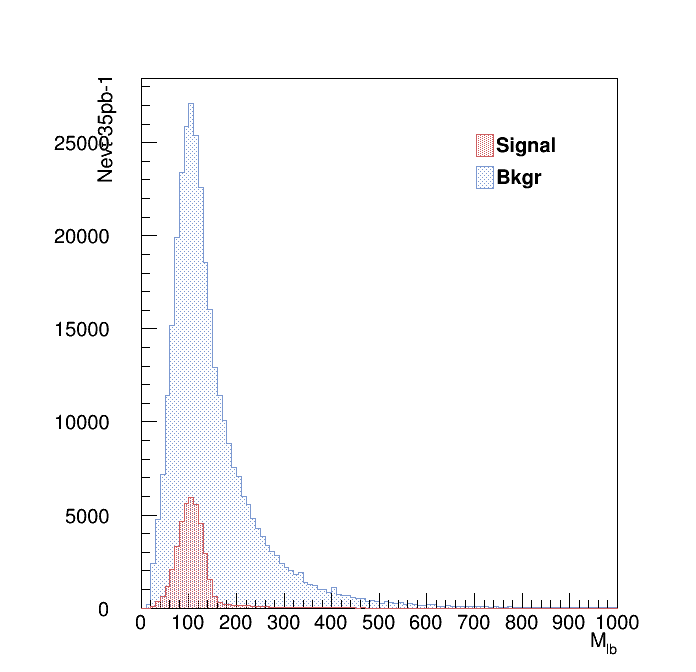
\includegraphics[width=0.5\textwidth]{/afs/ific.uv.es/user/p/pamarag/public/RedaccionTFM/Figuras/1d_only_signal_AND_bkg_tchannel_kine_mlb_tag.png}
\caption{$m_{l,b}$ distribution at preselection level for the electron channel.}
\label{Fig:mlbDistribution}
\end{figure}




\begin{figure}[h]
\centering
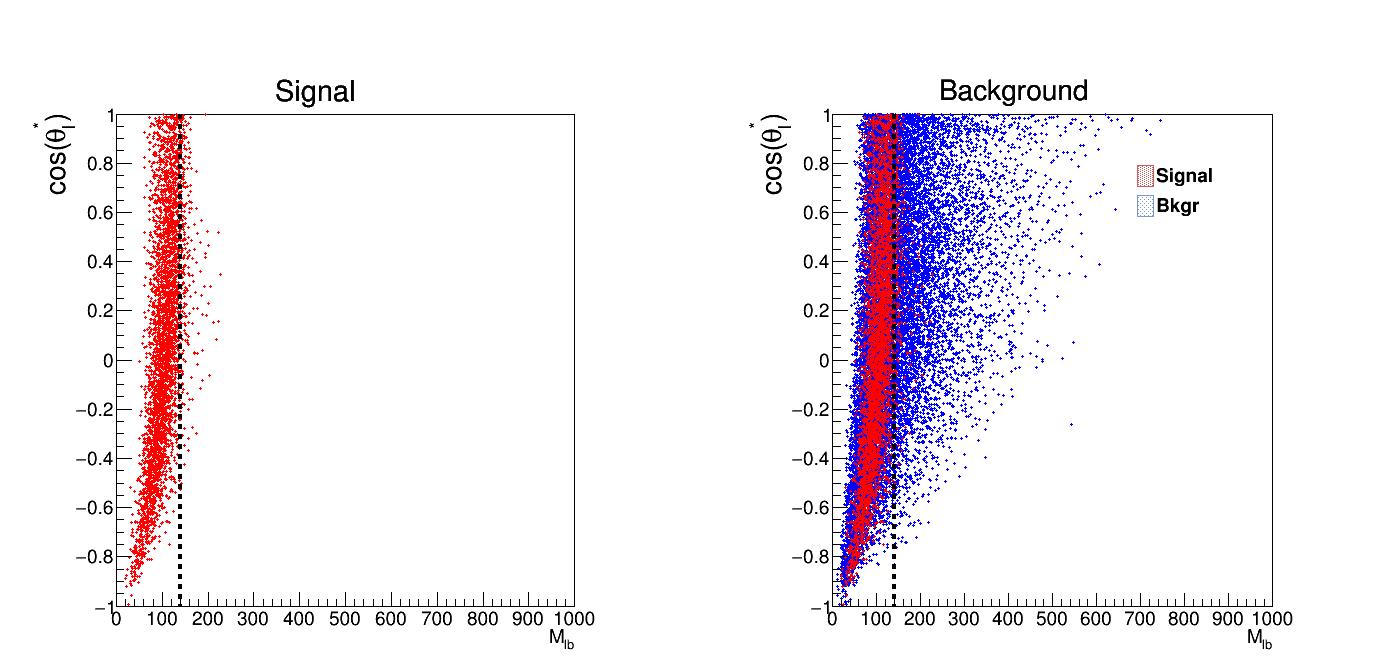
\includegraphics[width=0.95\textwidth]{/afs/ific.uv.es/user/p/pamarag/public/RedaccionTFM/Figuras/2d_signal_AND_bkg_tchannel_reco_tag_cos_S_kine_mlb_tag.png}
\caption{Scatter two-dimensional plot were the signal (background) has been scaled by a factor 0.1 (0.05) for aesthetic purposes of $\cos(\theta^{*})$ versus $m_{l,b}$ at preselection level for the electron channel. The doted line denotes the upper cut.}
\label{Fig:mlbVScosS}
\end{figure}

The event yields after applying the cut on $m_{l,b}$ are in Table~\ref{Table:mlbevents}, there can be seen that the significance and the $S/B$ have grown with respect to the preselection level. The significance has grown from 67 up to 75 and the $S/B$ from 0.121 to 0.181.
\begin{table} [h]
\begin{center}
%\resizebox{0.95\textwidth}{!}{%<---- To fit the table
\begin{tabular}{|c|c|c|c|c|} 
 \hline
 Process & Event yield & Bkg fraction \\ \hline
 $t$-channel & $36988 \pm 120 $ & - \\ 
 $Z$-jet, diboson & $5500 \pm 210 $&  2.7\% \\ 
 $W$+jets & $87948 \pm  1451$ & 43.1\%\\
 $t\bar{t}$& $80409 \pm 188$ & 39.4\%\\
 $Wt$ s-channel & $18061 \pm 98$ & 8.9\% \\
 Multijet&$12124\pm 107 $&5.9\%\\
 \hline
 Total & $241030 \pm 1490$ & - \\ \hline \hline
 S/B &\multicolumn{2}{|c|}{$0.181$} \\ \hline
 Significance &\multicolumn{2}{|c|}{$75$} \\ \hline
\end{tabular}
%}
\caption{Event yields and background fractions after preselection and requiring $m_{l,b} < 140$~GeV for MC 13~TeV samples. Electron channel.}
\label{Table:mlbevents}
\end{center}
\end{table}


\subsection{Optimisation of the \boldmath$m_{top}$ window}
%Comment for the cuts in $m_{top}$. \\
%After getting rid of a part of the sample using $m_{l,b}$, the next variable to be used it the mass of the top; which is expected to be very discriminant.
The second condition to be applied is over the mass of the top quark, its distribution is shown in Figure~\ref{Fig:topmassDistribution}. Cutting on $m_{top}$ is used to remove from the data events which do not have a real top: $Z$-jet, diboson, $W$+jets and multijet. But this is not helpful to clean the background of events such as $t\bar{t}$ or $Wt$ vertex in $s$-channel.

\begin{figure}[h]
\centering
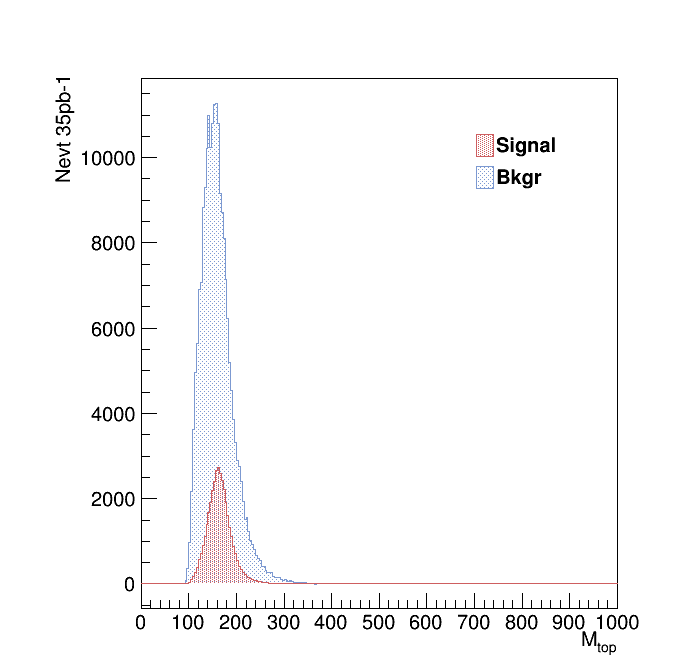
\includegraphics[width=0.55\textwidth]{/afs/ific.uv.es/user/p/pamarag/public/RedaccionTFM/Figuras/1d_only_signal_AND_bkg_tchannelmlb1_kine_topmass_tag.png}
\caption{$m_{top}$ distribution after preselection and $m_{l,b}$ cuts.}
\label{Fig:topmassDistribution}
\end{figure}

%When we want to set the cuts at first glance looking at a distribution (Figure~\ref{Fig:topmassDistribution}), the usual procedure is to normalize separately the signal and the background distributions so that both have the same scale. On the one hand, the peak of the background could displaced with respect to the theoretical value of $m_{top}$ because processes which does not include a real top quark ($W+jets$, $Z+jets$, diboson or multijets) are being considered, also, the width of the distribution is larger than for the signal due to the fact that we are combining the distribution of different processes (sum of different gaussians). On the other hand, the distribution corresponding to the signal will be centred in the expected value of the top mass because we are simulating processes with a single top. Therefore, we will have two gaussians of similar heigh but the background one is wider than the signal and may have a different mean value. This scenario allows to put an upper and/or a lower cut in the variable just taking a look to the histogram with the two distributions.
%Instead of this methodology, in this case, 2D histograms (Figure~\ref{Fig:m(top)3D}) showing the significance and the $S/B$ ratio as a function of the lower and the upper cuts have been created. Following a criteria of maximum significance first and maximum $S/B$ ratio second we the optimum upper and lower boundaries of the $m_{top}$ variable are sat.

Starting from the one dimensional distribution of $m_{top}$ we have built two dimensional maps of significance and $S/B$ by sweeping simultaneously the lower and the upper requirement on $m_{top}$ in the ranges shown in the X and Y axes of Figure~\ref{Fig:m(top)3D}. At a given point ($m_{top}(lower)$, $m_{top}(upper)$) of these two dimensional maps, significance and $S/B$ have been obtained from the integral of the one dimensional distributions signal and background distributions in the range: $m_{top}(lower) < m_{top} < m_{top}(upper)$.

\begin{figure}[h]
\centering
\subfloat[Significance]{
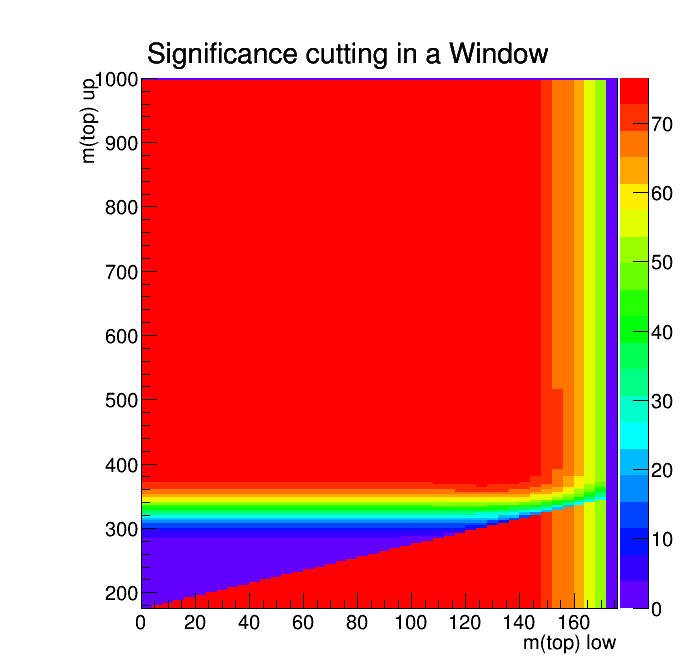
\includegraphics[width=0.45\textwidth]{/afs/ific.uv.es/user/p/pamarag/public/RedaccionTFM/Figuras/2D_Significance_Window_tchannelmlb1_kine_topmass_tag.png}
}
\subfloat[$S/B$ ratio]{
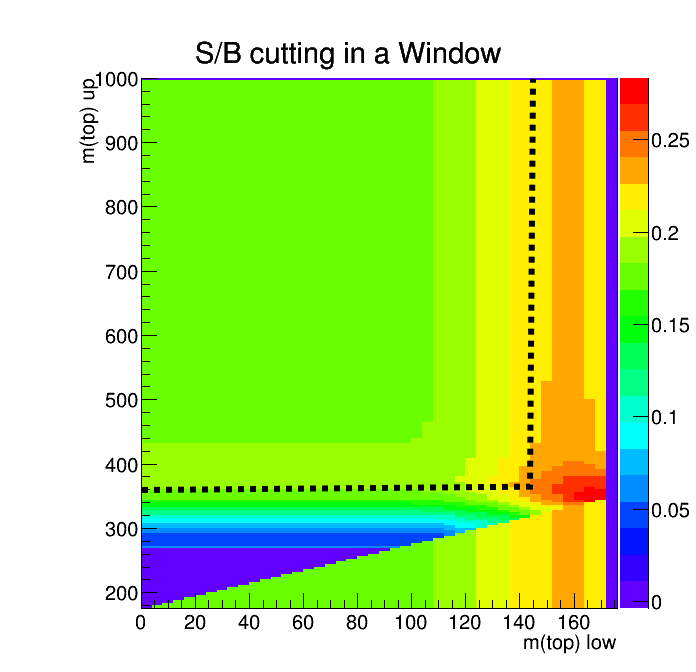
\includegraphics[width=0.45\textwidth]{/afs/ific.uv.es/user/p/pamarag/public/RedaccionTFM/Figuras/2D_SignificanceStoB_Window_tchannelmlb1_kine_topmass_tagDOTED.png}
%Poner la figura que toca. Intentar plotear dos figuras en un único canvas.
}
\caption{Two dimensional histograms showing significance and $S/N$ ratio for $m_{top}$ with lower and upper cuts. The doted line in (b) delimit the area in which the significance is maximum.}
\label{Fig:m(top)3D}
\end{figure}

In Figure~\ref{Fig:m(top)3D}-(a), can be seen that the maximal significance criteria is satisfied with any upper cut above 360 GeV and lower below 147 GeV. Then we pay attention at Figure~\ref{Fig:m(top)3D}-(b) to look for the point that, satisfying the previous condition, maximises the $S/B$ ratio. Scanning the values of significance and $S/B$ for all bins between 140~GeV and 160~GeV for the lower cut and 350~GeV to 450~GeV for the upper, we find that the optimum limits for the $m_{top}$ are:
\begin{align*}
m_{top}(lower) &= 142 \textrm{ GeV}\\
m_{top}(upper) &= 418 \textrm{ GeV}
\end{align*}
The peak of the top mass is on its theoretical value, 175 GeV, which lays inside the window defined by the cuts. Table~\ref{Table:mtopevents} shows the event yields after demanding that the conditions $m_{l,b}<140$~GeV and $m_{top} \in [142,$ $148]$ are satisfied. As expected, all backgrounds that do not contain a real top have lost relevance regarding the background fraction: the $Z$-jet and diboson from 2.7\% to 2.2\%, the $W$+jets from 43.1\% to 38.1\% and the multijet from 5.9\% to 4.1\%.

\begin{table} [h]
\begin{center}
%\resizebox{0.95\textwidth}{!}{%<---- To fit the table
\begin{tabular}{|c|c|c|c|c|} 
 \hline
 Process & Event yield & Bkg fraction \\ \hline
 $t$-channel & $30477 \pm 109 $ & - \\ 
 $Z$-jet, diboson & $3094 \pm 134 $& 2.2\% \\ 
 $W$+jets & $53180 \pm  1085$ & 38.4\%\\
 $t\bar{t}$& $62880 \pm 166$ & 45.4\%\\
 $Wt$ s-channel & $13780 \pm 86$ & 9.9\% \\
 Multijet&$5675 \pm 79 $&4.1\%\\
 \hline
 Total & $169086 \pm 1117$ & - \\ \hline \hline
 S/B &\multicolumn{2}{|c|}{$0.220$} \\ \hline
 Significance &\multicolumn{2}{|c|}{$74$} \\ \hline
\end{tabular}
%}
\caption{Event yields after preselection, $m_{l,b} < 140$~GeV and $142 <m_{top} < 418$~GeV requirements for 13~TeV MC samples. Only the electron channel is considered.}
\label{Table:mtopevents}
\end{center}
\end{table}

%\begin{center}
%\begin{table} [htb]
%\resizebox{!}{0.46\textheight}{
%\begin{tabular}{|c|c|c|}
% \hline
% Cut(upper, lower)GeV & Significance & $S/B$ \\ \hline
%$142$, $354$& $65.29$&$0.231$ \\ 
%$142$, $358$& $67.72$&$0.232$ \\
%$142$, $362$& $69.66$&$0.233$ \\ 
%$142$, $366$& $71.23$&$0.234$ \\ 
%$142$, $370$& $72.38$&$0.234$ \\ 
%$142$, $374$& $73.26$&$0.233$ \\
%$142$, $378$& $73.83$&$0.232$ \\
%$142$, $382$& $74.14$&$0.231$ \\
%$142$, $386$& $74.36$&$0.229$ \\
%$142$, $390$& $74.54$&$0.228$ \\
%$142$, $394$& $74.68$&$0.227$ \\
%$142$, $398$& $74.71$&$0.225$ \\
%$142$, $402$& $74.79$&$0.225$ \\
%$142$, $406$& $74.84$&$0.224$ \\
%$142$, $410$& $74.86$&$0.223$ \\
%$142$, $414$& $74.86$&$0.222$ \\
%$142$, $418$& $74.87$&$0.222$ \\
%$142$, $422$& $74.86$&$0.221$ \\
%$142$, $426$& $74.86$&$0.221$ \\
%$142$, $430$& $74.87$&$0.220$ \\
%$142$, $434$& $74.86$&$0.220$ \\
%$142$, $438$& $74.86$&$0.220$ \\
%$142$, $442$& $74.85$&$0.219$ \\
%$142$, $446$& $74.83$&$0.219$ \\
%$146$, $354$& $63.90$&$0.241$ \\
%$146$, $358$& $66.39$&$0.242$ \\
%$146$, $362$& $68.37$&$0.242$ \\
%$146$, $366$& $69.97$&$0.243$ \\
%$146$, $370$& $71.15$&$0.242$ \\
%$146$, $374$& $72.03$&$0.241$ \\
%$146$, $378$& $72.60$&$0.240$ \\
%$146$, $382$& $72.91$&$0.238$ \\
%$146$, $386$& $73.12$&$0.236$ \\
%$146$, $390$& $73.29$&$0.235$ \\
%$146$, $394$& $73.43$&$0.233$ \\
%$146$, $398$& $73.45$&$0.232$ \\
%$146$, $402$& $73.53$&$0.231$ \\
%$146$, $406$& $73.57$&$0.230$ \\
%$146$, $410$& $73.59$&$0.229$ \\
%$146$, $414$& $73.58$&$0.228$ \\
%$146$, $418$& $73.59$&$0.228$ \\
%$146$, $422$& $73.58$&$0.227$ \\~GeV
%$146$, $426$& $73.58$&$0.226$ \\
%$146$, $430$& $73.58$&$0.226$ \\
%$146$, $434$& $73.57$&$0.226$ \\
%$146$, $438$& $73.56$&$0.225$ \\
%$146$, $442$& $73.56$&$0.225$ \\
%$146$, $446$& $73.54$&$0.225$ \\
%$150$, $354$& $61.64$&$0.248$ \\
%$150$, $358$& $64.22$&$0.248$ \\
%$150$, $362$& $66.26$&$0.249$ \\
%$150$, $366$& $67.92$&$0.249$ \\
%$150$, $370$& $69.12$&$0.248$ \\
%$150$, $374$& $70.03$&$0.247$ \\
%$150$, $378$& $70.61$&$0.245$ \\
%$150$, $382$& $70.91$&$0.243$ \\
%$150$, $386$& $71.13$&$0.241$ \\
%$150$, $390$& $71.30$&$0.239$ \\
%$150$, $394$& $71.43$&$0.238$ \\
%$150$, $398$& $71.45$&$0.236$ \\
%$150$, $402$& $71.53$&$0.235$ \\
%$150$, $406$& $71.57$&$0.234$ \\
%$150$, $410$& $71.58$&$0.233$ \\
%$150$, $414$& $71.57$&$0.232$ \\
%$150$, $418$& $71.58$&$0.231$ \\
%$150$, $422$& $71.57$&$0.230$ \\
%$150$, $426$& $71.56$&$0.230$ \\
%$150$, $430$& $71.56$&$0.229$ \\
%$150$, $434$& $71.55$&$0.229$ \\
%$150$, $438$& $71.54$&$0.229$ \\
%$150$, $442$& $71.54$&$0.228$ \\
%$150$, $446$& $71.52$&$0.228$ \\


%\end{tabular}
%}
%\caption{Scan}
%\end{table}
%\end{center}
\subsection{\boldmath$\Delta \eta_{j,top}$ and \boldmath$|\eta_j|$ triangular cut}
In the case of the variables $\Delta \eta_{j,top}$ and $|\eta_j|$ (Figure~\ref{Fig:Detajt&etaj}), the two-dimensional correlation shown in Figure~\ref{Fig:Triangular} suggested a triangular cut of the form: $|\eta_j| > \eta_{j0} - \Delta\eta_{j,top}$, with $\eta_{j0}$ to be optimised. The event yields, background fractions, significances and $S/B$ ratios, obtained after applying the preselection, $m_{l,b}$, $m_{top}$ and triangular cut are shown in Table~\ref{Table:ABCtriang} for different values of $\eta_{j0}$. For maximasing the significance, $\eta_{j0}=3.0$ is the best choice but, nevertheless, we are using we take $\eta_{j0}=3.5$ because we have a gain in $S/B$ of 19\% compared to the $\eta_{j0}=3.0$ case by only loosing a 1.3\% of significance. The $S/B$ ratio has been doubled with this new cut.

%The distribution of events over those variables and the correlation of $\Delta \eta_{j,top}$ and $|\eta_j|$ is shown in Figure~\ref{Fig:Detajt&etaj} and Figure~\ref{Fig:Triangular} respectively. Looking at Figure~\ref{Fig:Triangular}, can be noticed that a triangular cut that removes the events with $|\eta_j| < \eta_{j0} - \Delta\eta_{j,top}$ (with $\eta_{j0}$ to be optimised) would remove significantly much more background than signal. The proposed cuts and the obtained event yields are shown in Table~\ref{Table:ABCtriang}. As can be seen, $\eta_{j0}=3.0$ optimises the significance, which is the statistical parameter in which we are focused. Nevertheless, we take $\eta_{j0}=3.5$ because we have a gain  in $S/B$ of 19\% compared to the $\eta_{j0}=3.0$ case by only  loosing a 1.3\% of significance.

\begin{figure}[h]
\centering
\subfloat[$\Delta \eta_{j,top}$]{
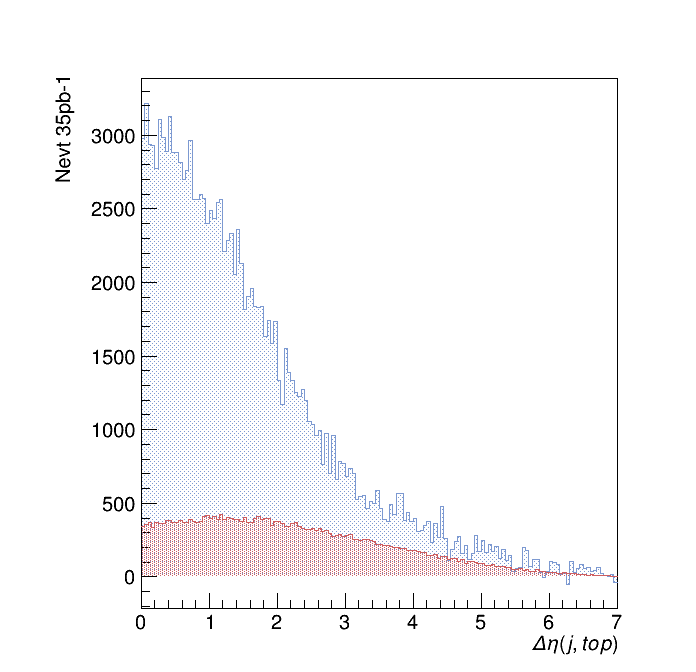
\includegraphics[width=0.45\textwidth]{/afs/ific.uv.es/user/p/pamarag/public/RedaccionTFM/Figuras/1d_only_signal_AND_bkg_tchannelmlbmtop_dEtajtop.png}
}
\subfloat[$|\eta_j|$]{
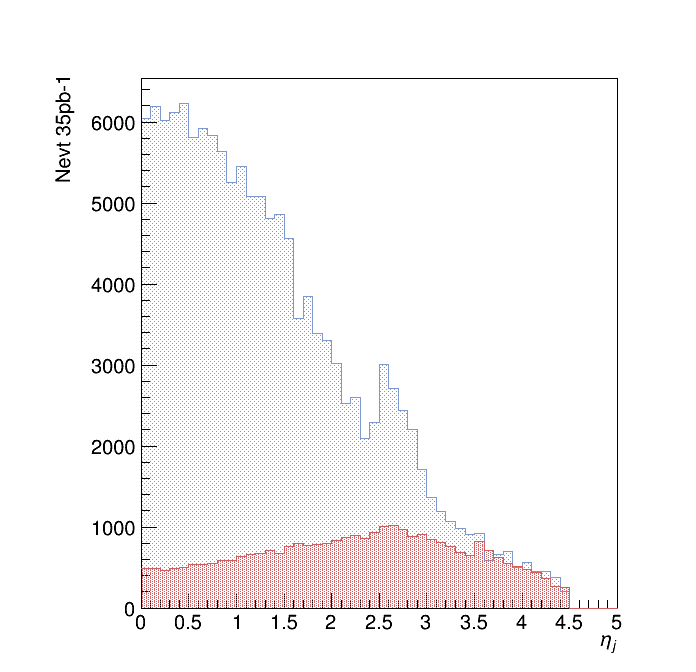
\includegraphics[width=0.45\textwidth]{/afs/ific.uv.es/user/p/pamarag/public/RedaccionTFM/Figuras/1d_only_signal_AND_bkg_tchannelmlbmtop_kine_eta_lightjet_tag.png}
%Poner la figura que toca. Intentar plotear dos figuras en un único canvas.
}
\caption{Distribution of (a) $\Delta \eta_{j,top}$ and (b) $|\eta_j|$ after applying the cuts in $m_{l,b}$ and $m_{top}$. Electron channel. The red area is the signal wihile the blue is the background.} 
\label{Fig:Detajt&etaj}
\end{figure}
%At this point I could show, instead of the absolute value of the $\eta_j$ (kine\_eta\_lightjet\_tag), the positive and negative axis of $\eta_j$ (reco\_top\_eta\_tag). 

\begin{figure}[h]
\centering
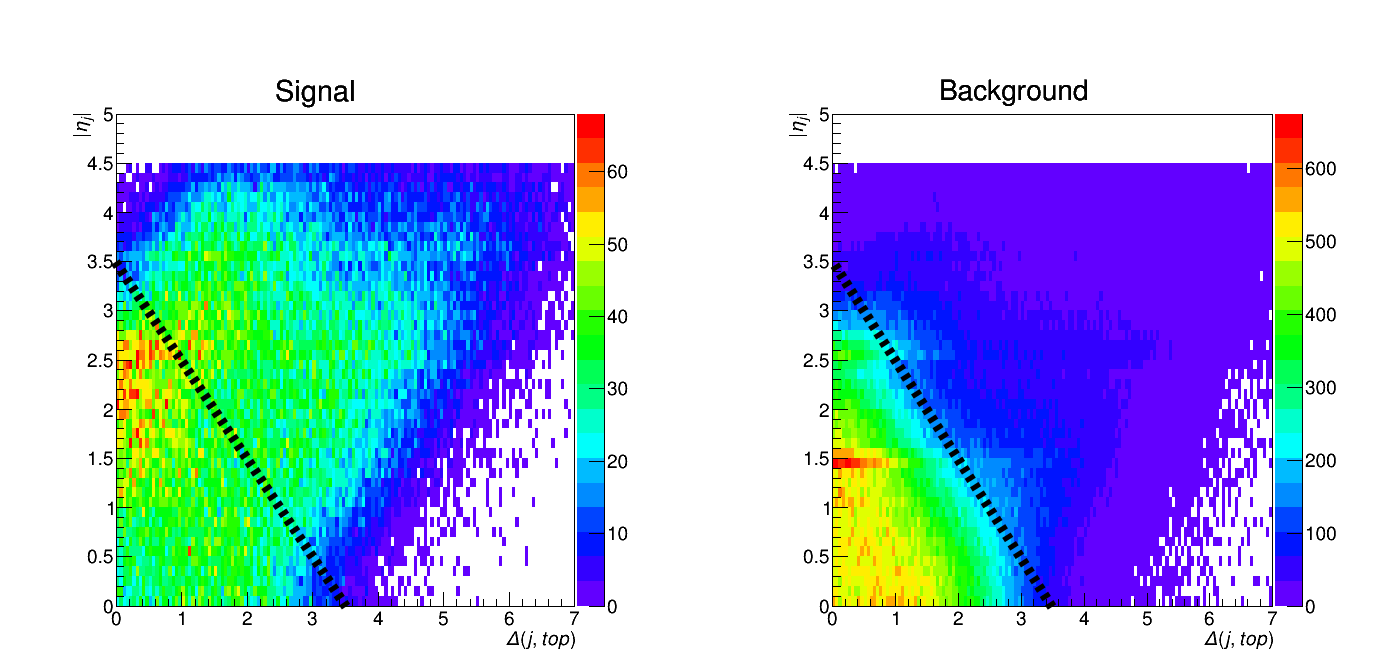
\includegraphics[width=1\textwidth]{/afs/ific.uv.es/user/p/pamarag/public/RedaccionTFM/Figuras/2d_signal_AND_bkg_tchannelmlbmtop_kine_eta_lightjet_tag_dEtajtopDOTED.png}
\caption{Two-dimensional correlation between $|\eta_j|$ and $\Delta\eta_{j,top}$ after the cuts in $m_{top}$ and $m_{l,b}$ have been applied. The area below the doted line is removed from the selection.}
\label{Fig:Triangular}
\end{figure}

\begin{table} [h]
\begin{center}
%\resizebox{0.95\textwidth}{!}{%<---- To fit the table
\begin{tabular}{|c||c|c|c|} 
 \hline
  & \multicolumn{3}{|c|}{Event yields} \\ \cline{2-4}
 Process & $\eta_{j0}=2.8$ & $\eta_{j0}=3.0$ & $\eta_{j0}=3.5$ \\ \hline
 $t$-channel & $23008 \pm 94 $ & $ 21942\pm 92 $& $ 19259\pm 86 $\\ 
 $Z$-jet, diboson & $ 1722\pm 110 $& $1547 \pm 106 $& $1126 \pm 93 $ \\ 
 $W$+jets & $ 26521\pm 924  $ & $ 23692\pm 901 $& $18422 \pm 809 $\\
 $t\bar{t}$& $ 23914\pm 103  $ & $20706 \pm  96$& $14498 \pm 80 $\\
 $Wt$ s-channel & $4677 \pm 51 $ & $3944 \pm 46 $& $2687 \pm 38 $\\
 Multijet&$4292 \pm 72 $ & $3957 \pm 69$& $2961 \pm 58 $\\
 \hline
 Total & $84134 \pm 946$ & $75788 \pm 921$ & $58954 \pm 825$ \\ \hline \hline
 S/B & 0.376 & 0.408 & 0.485 \\ \hline
 Significance & 79 & 80 & 79 \\ \hline
\end{tabular}
%}
\caption{Keeping events with $m_{l,b} < 140$ GeV and $142 < m_{top} < 418$ GeV and a cut of the form $|\eta_j| > \eta_{j0} - \Delta\eta_{j,top}$ for 13 TeV samples.}
\label{Table:ABCtriang}
\end{center}
\end{table}

\subsection{Two dimensional optimisation of \boldmath$H_{T}$ and \boldmath$m_{j,top}$, requirements}
%\textbf{Reproducir mapas de Susana}

The $S/B$ and significance obtained after preselection, $m_{l,b}< 140$~GeV, 142~GeV~$ < m_{top} < 418$~GeV and $|\eta_j| > 3.5 - \Delta\eta_{j,top}$ could be improved further improved with further requirements. At this stage, we consider a two dimensional optimisation of two variables that do not depend on kinematic properties of individual top quark decay products: $H_{T}$ and $m_{j,top}$.

Starting from the two dimensional distribution of $m_{j,top}$ versus $H_{T}$ we have built two dimensional maps of significance and $S/B$ using a two dimensional integration by sweeping simultaneously: $H_{T} > H_{T}(min)$ and $m_{j,top}> m_{j,top}(min)$.

Later, we maximise the significance by iterating over the bins of the previous significance map in Figure~\ref{Fig:MjtHt_Sig_SB} searching for the maximum value of significance and keeping a fixed working point of minimum $S/B$ required.

\begin{figure}[htb]
\centering
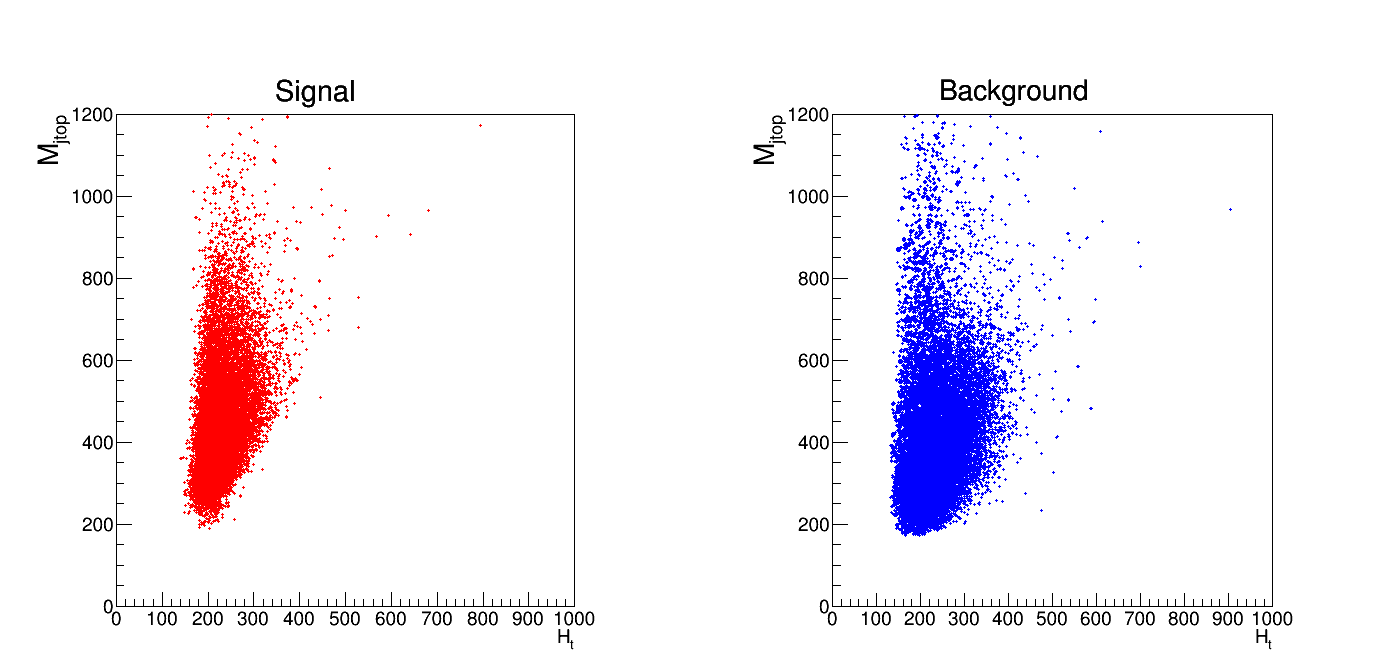
\includegraphics[width=0.99\textwidth]{/afs/ific.uv.es/user/p/pamarag/public/RedaccionTFM/Figuras/2d_signal_AND_bkg_selection13tevH_Mjtop_kine_ht_tag.png}
\caption{Correlation between $H_{T}$ and $m_{j,top}$ for 13~TeV MC samples after the preselection, $m_{l,b}$, $m_{top}$, $\Delta\eta_{j, top}$ and $|\eta_j|$ requirements are applied. Electron channel. In this scatter two dimensional plot the signal has been scaled by a factor 0.1 and the background by a factor 0.05 for aesthetic purposes.}
\label{Fig:MjtHt_Dist}
\end{figure}

\begin{figure}[htb]
\centering
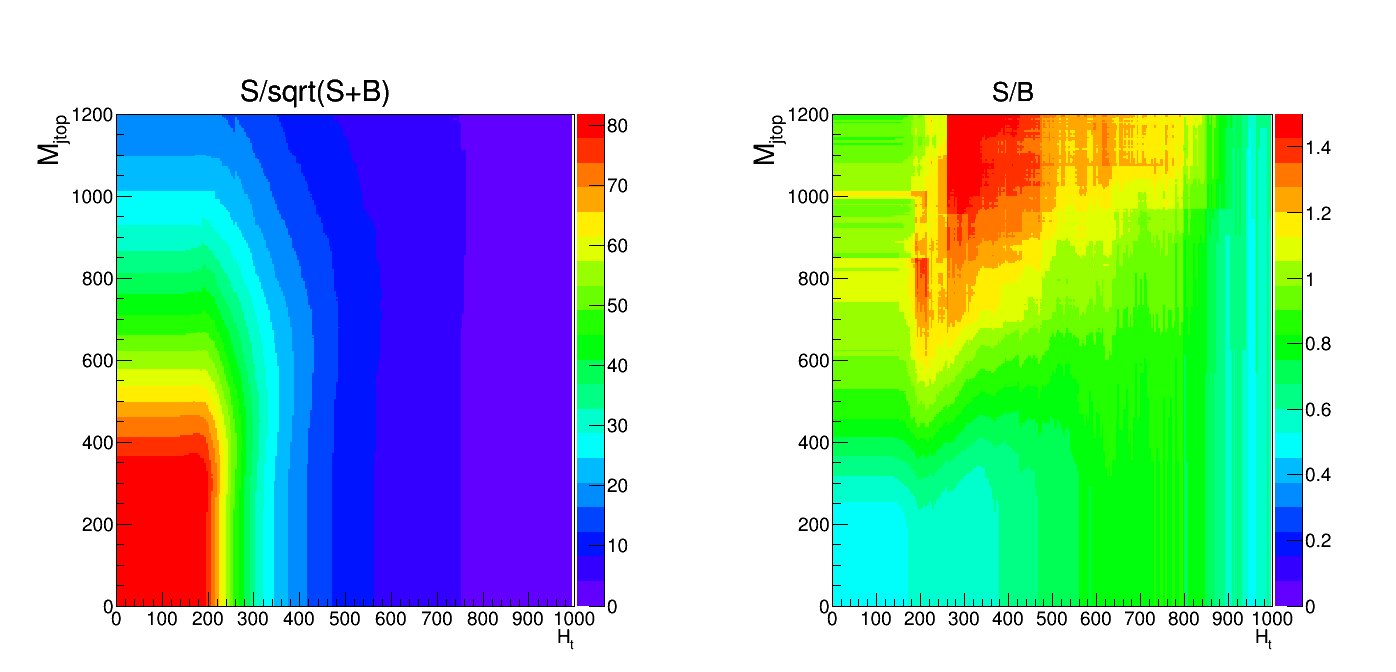
\includegraphics[width=0.99\textwidth]{/afs/ific.uv.es/user/p/pamarag/public/RedaccionTFM/Figuras/2d_Significance_StB_selection13tevH_Mjtop_kine_ht_tag.png}
\caption{Maps of significance and $S/B$ depending on the $H_{T}(min)$ and $m_{j,top}(min)$ used for the cuts. The preselection, $m_{l,b}$, $m_{top}$, $\Delta\eta_{j, top}$ and $|\eta_j|$ requirements, are also considered.}
\label{Fig:MjtHt_Sig_SB}
\end{figure}

Afterwards, we keep various fixed working points of minimum $S/B$ and maximise the significance. % If there are several points ($H_{T}(min)$, $m_{j,top}(min)$) in that have same significance, the criterion of maximising the $S/B$ is applied.
 From the map of significances, these points are identified for five boundary cases of minimum $S/B$: 0, 0.65, 1, 1.2 and 1.4. See Table~\ref{Table:MjtHtMisc}. 

\begin{table} [htb]
\begin{center}
%\resizebox{0.95\textwidth}{!}
\caption{Significances and $S/B$ ratios for 13~TeV MC samples depending on the cuts applied over $m_{j,top}$ and $H_{T}$ for different cases of minimum $S/B$. The preselection, $m_{l,b}$, $m_{top}$, $\Delta\eta_{j, top}$ and $|\eta_j|$ requirements, are applied.} 
\label{Table:MjtHtMisc}
\end{center}
\end{table}

The significances and $S/B$ from Table~\ref{Table:MjtHtMisc} are directly obtained from Figure~\ref{Fig:MjtHt_Sig_SB}. With the several optimised selections for the different requirements of minimum $S/B$, selection regions are defined and their event yields are shown in Table~\ref{Table:FINAL}. There can be seen that the predictions of significance and $S/B$ from Table~\ref{Table:MjtHtMisc} are in agreement with the calculations with the event yields of Table~\ref{Table:FINAL}. 

\begin{table} [htb]
\begin{center}
%\resizebox{0.95\textwidth}{!}{%<---- To fit the table
\begin{tabular}{|c|c|c|c|c|c|} 
\hline
& \multicolumn{5}{|c|}{Event yields. ($H_T (min)$, $m_{j,top}(min)$)} \\ \cline{2-6}
Process & (168, 284) & (176, 316) & (192, 512) & (212, 608) & (192, 824) \\ \hline
$t$-channel & $17929 \pm 83$ & $16604 \pm 80$ & $8043 \pm 57$ & $4943 \pm 45$&$2376\pm 31$ \\
$Z$-jet, diboson & $841 \pm 85$  & $658\pm 74$ & $192\pm 49$  & $50\pm 12$ &$13 \pm 10$ \\
$W$+jets & $13189 \pm 704$ & $10996\pm 654$ & $3267 \pm 389$ &$1532\pm 326$&$622\pm 314$\\
$t\bar{t}$ & $12088\pm 74$ & $10564\pm 69$ & $3456\pm 40$ &$1963\pm 30$ & $729\pm 19$\\
$Wt$ $s$-channel & $2052 \pm 33$ & $1684\pm 29$ & $508 \pm 16$ & $277 \pm 13$ & $106 \pm 7$ \\
Multijet & $1795 \pm 45$ & $1472\pm 40$ & $572\pm 26$ & $290\pm 19$ & $220\pm 18$\\ \hline 
Total & $47895 \pm 720$ & $41979\pm 668$ & $16038\pm 399$ &$9056\pm 332$& $4065\pm 317$\\ \hline \hline
Significance & 82 & 81 & 64 & 52 & 37 \\ \hline
$S/B$ & 0.598 & 0.654 & 1.006 & 1.202 & 1.406 \\ \hline


\end{tabular}
%}
\caption{Event yields for 13~TeV MC samples after applying the preselection requirements, $m_{l,b} < 140$~GeV, $142 < m_{top} < 418$~GeV, $|\eta_j| > 3.5-\Delta\eta_{j,top}$ and $m_{j,top}$ and $H_{T}$ cuts. Each columns refers to a different set of lower cuts in $m_{j,top}$ and $H_{T}$ according to the optimisation of Table~\ref{Table:MjtHtMisc}.} 
\label{Table:FINAL}
\end{center}
\end{table}

\clearpage

